\chapter{Large area device simulation}
\label{ref:la}
Gpvdm primarily focuses on drift diffusion modelling of small area device such as solar cells and OFETs. Drift and diffusion simulations are good at describing the microscopic operation of devices. They allow you to understand how carriers, potential and recombination interact on the nanometer scale.  However, sometimes one wants to simulate large area devices such as printed substrates spanning over many square centimetres.  For this type of simulation one needs to use less detailed and more efficient circuit models, this section describes how to do that.

Related YouTube videos:
\begin{figure}[H]

\begin{tabular}{ c l }


\includegraphics[width=0.05\textwidth]{./images/youtube.png}

&
\href{https://www.youtube.com/watch?v=XpGr9C_gr7E}{Tutorial on designing large area contacts for flexible electronics}\
\\

\includegraphics[width=0.05\textwidth]{./images/youtube.png}

&
\href{https://www.youtube.com/watch?v=ObBJIE9TmYo}{Understanding Printed Hexagonal Contacts for Large Area Solar Cells}

\end{tabular}
\end{figure}



\section{Designing contacts for large area devices}
A common problem is designing large area contacts for solar cells.  This paper \cite{solak2021understanding} gives an overview of such a problem.   To start designing large area contacts open the new simulation window in the file ribbon, and select the \emph{Large area hexagonal contact} simulation (see figure \ref{fig:newsimlargeareacontact}).  Once you have opened it you should get a window which looks like figure \ref{fig:basecontactsimulation}.  This simulation consists for a hexagonal solver contact printed on top of a PEDOT substrate.  We are going to find out how the resistance of this contact varies as a function of position.




\begin{figure}[H]
\centering
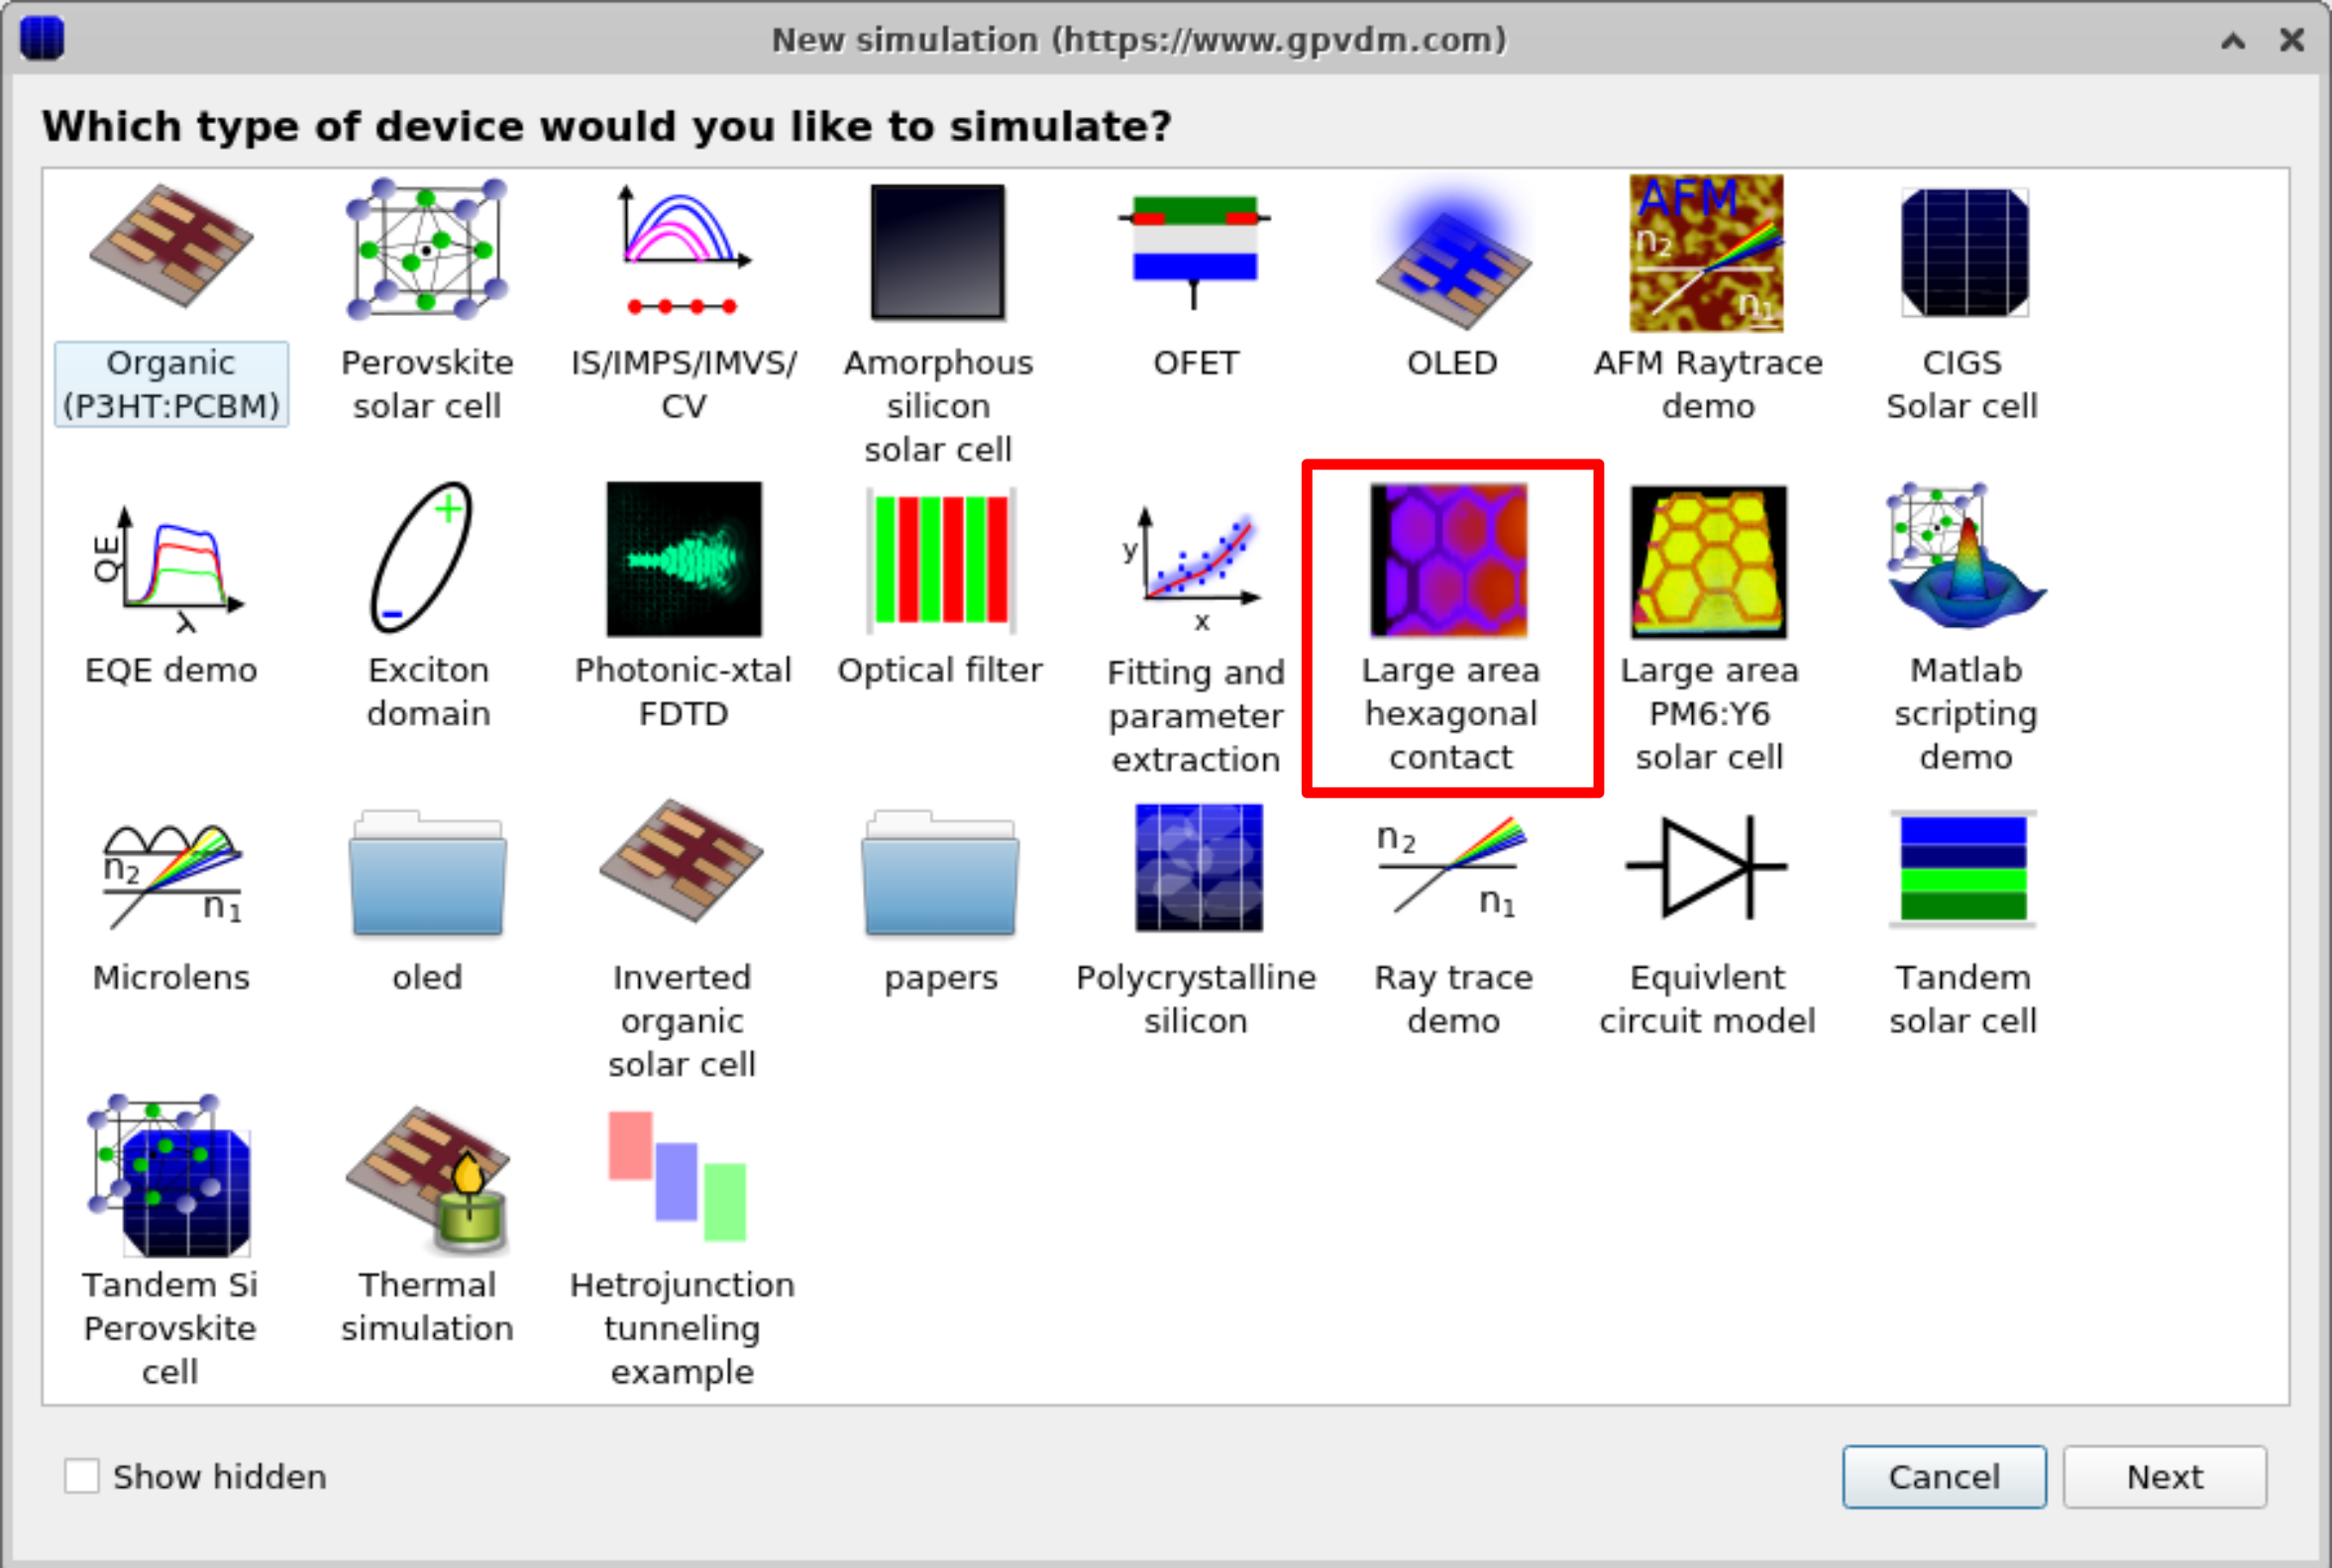
\includegraphics[width=\textwidth]{./images/la_0.png}
\caption{Selecting the large area contact simulation}
\label{fig:newsimlargeareacontact}
\end{figure}

\begin{figure}[H]
\centering
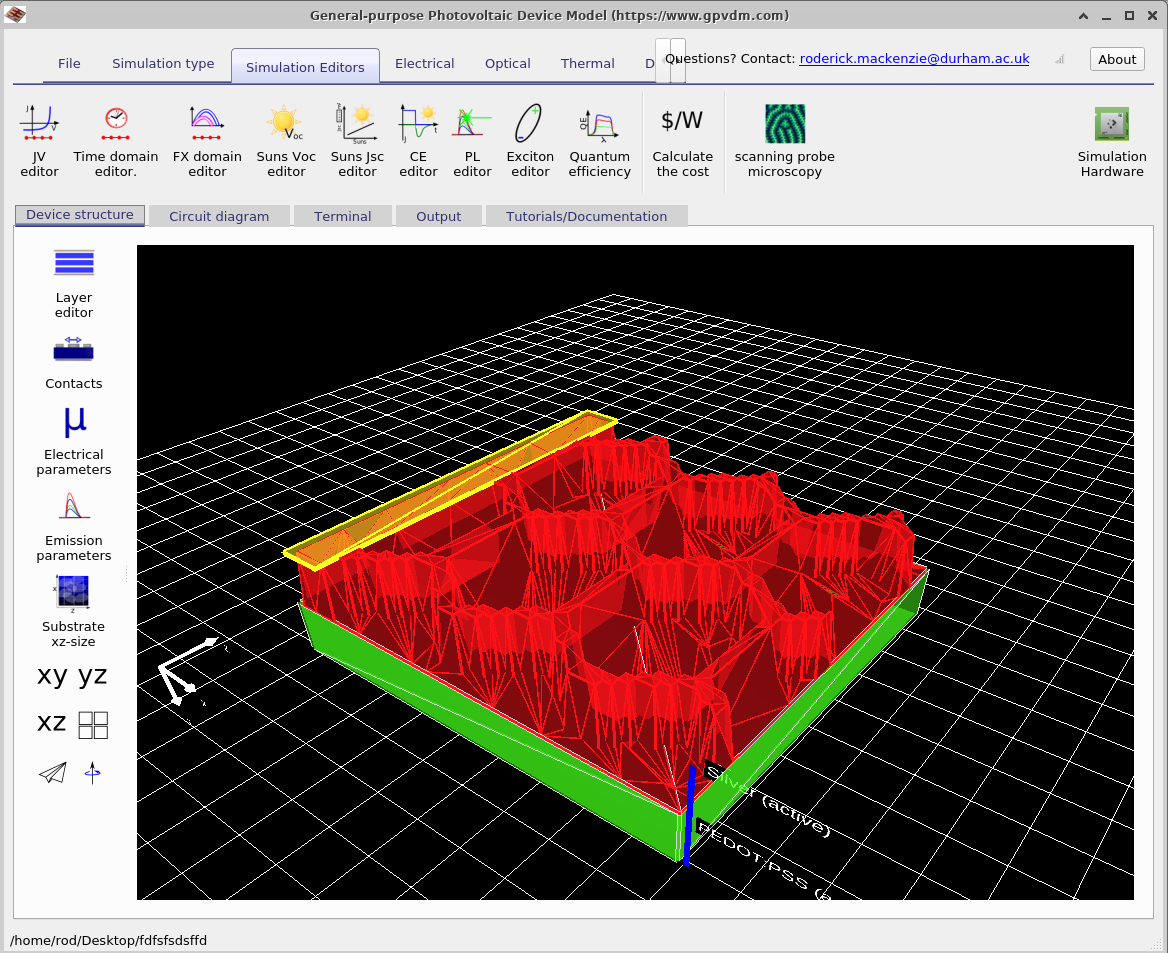
\includegraphics[width=\textwidth]{./images/la_1.png}
\caption{A 3D image of the contact printed contact.}
\label{fig:basecontactsimulation}
\end{figure}

The next step in the simulation is to build a network of resistors which approximates the shape of the contact. To do this select the Circuit diagram tab and then click the refresh button.  This will build a resistor network of the shape shown in the device structure tab, see figure \ref{fig:threedcircuitmesh}. Here you can zoom in and examine the individual resistors, each line represents a resistor.

\begin{figure}[H]
\centering
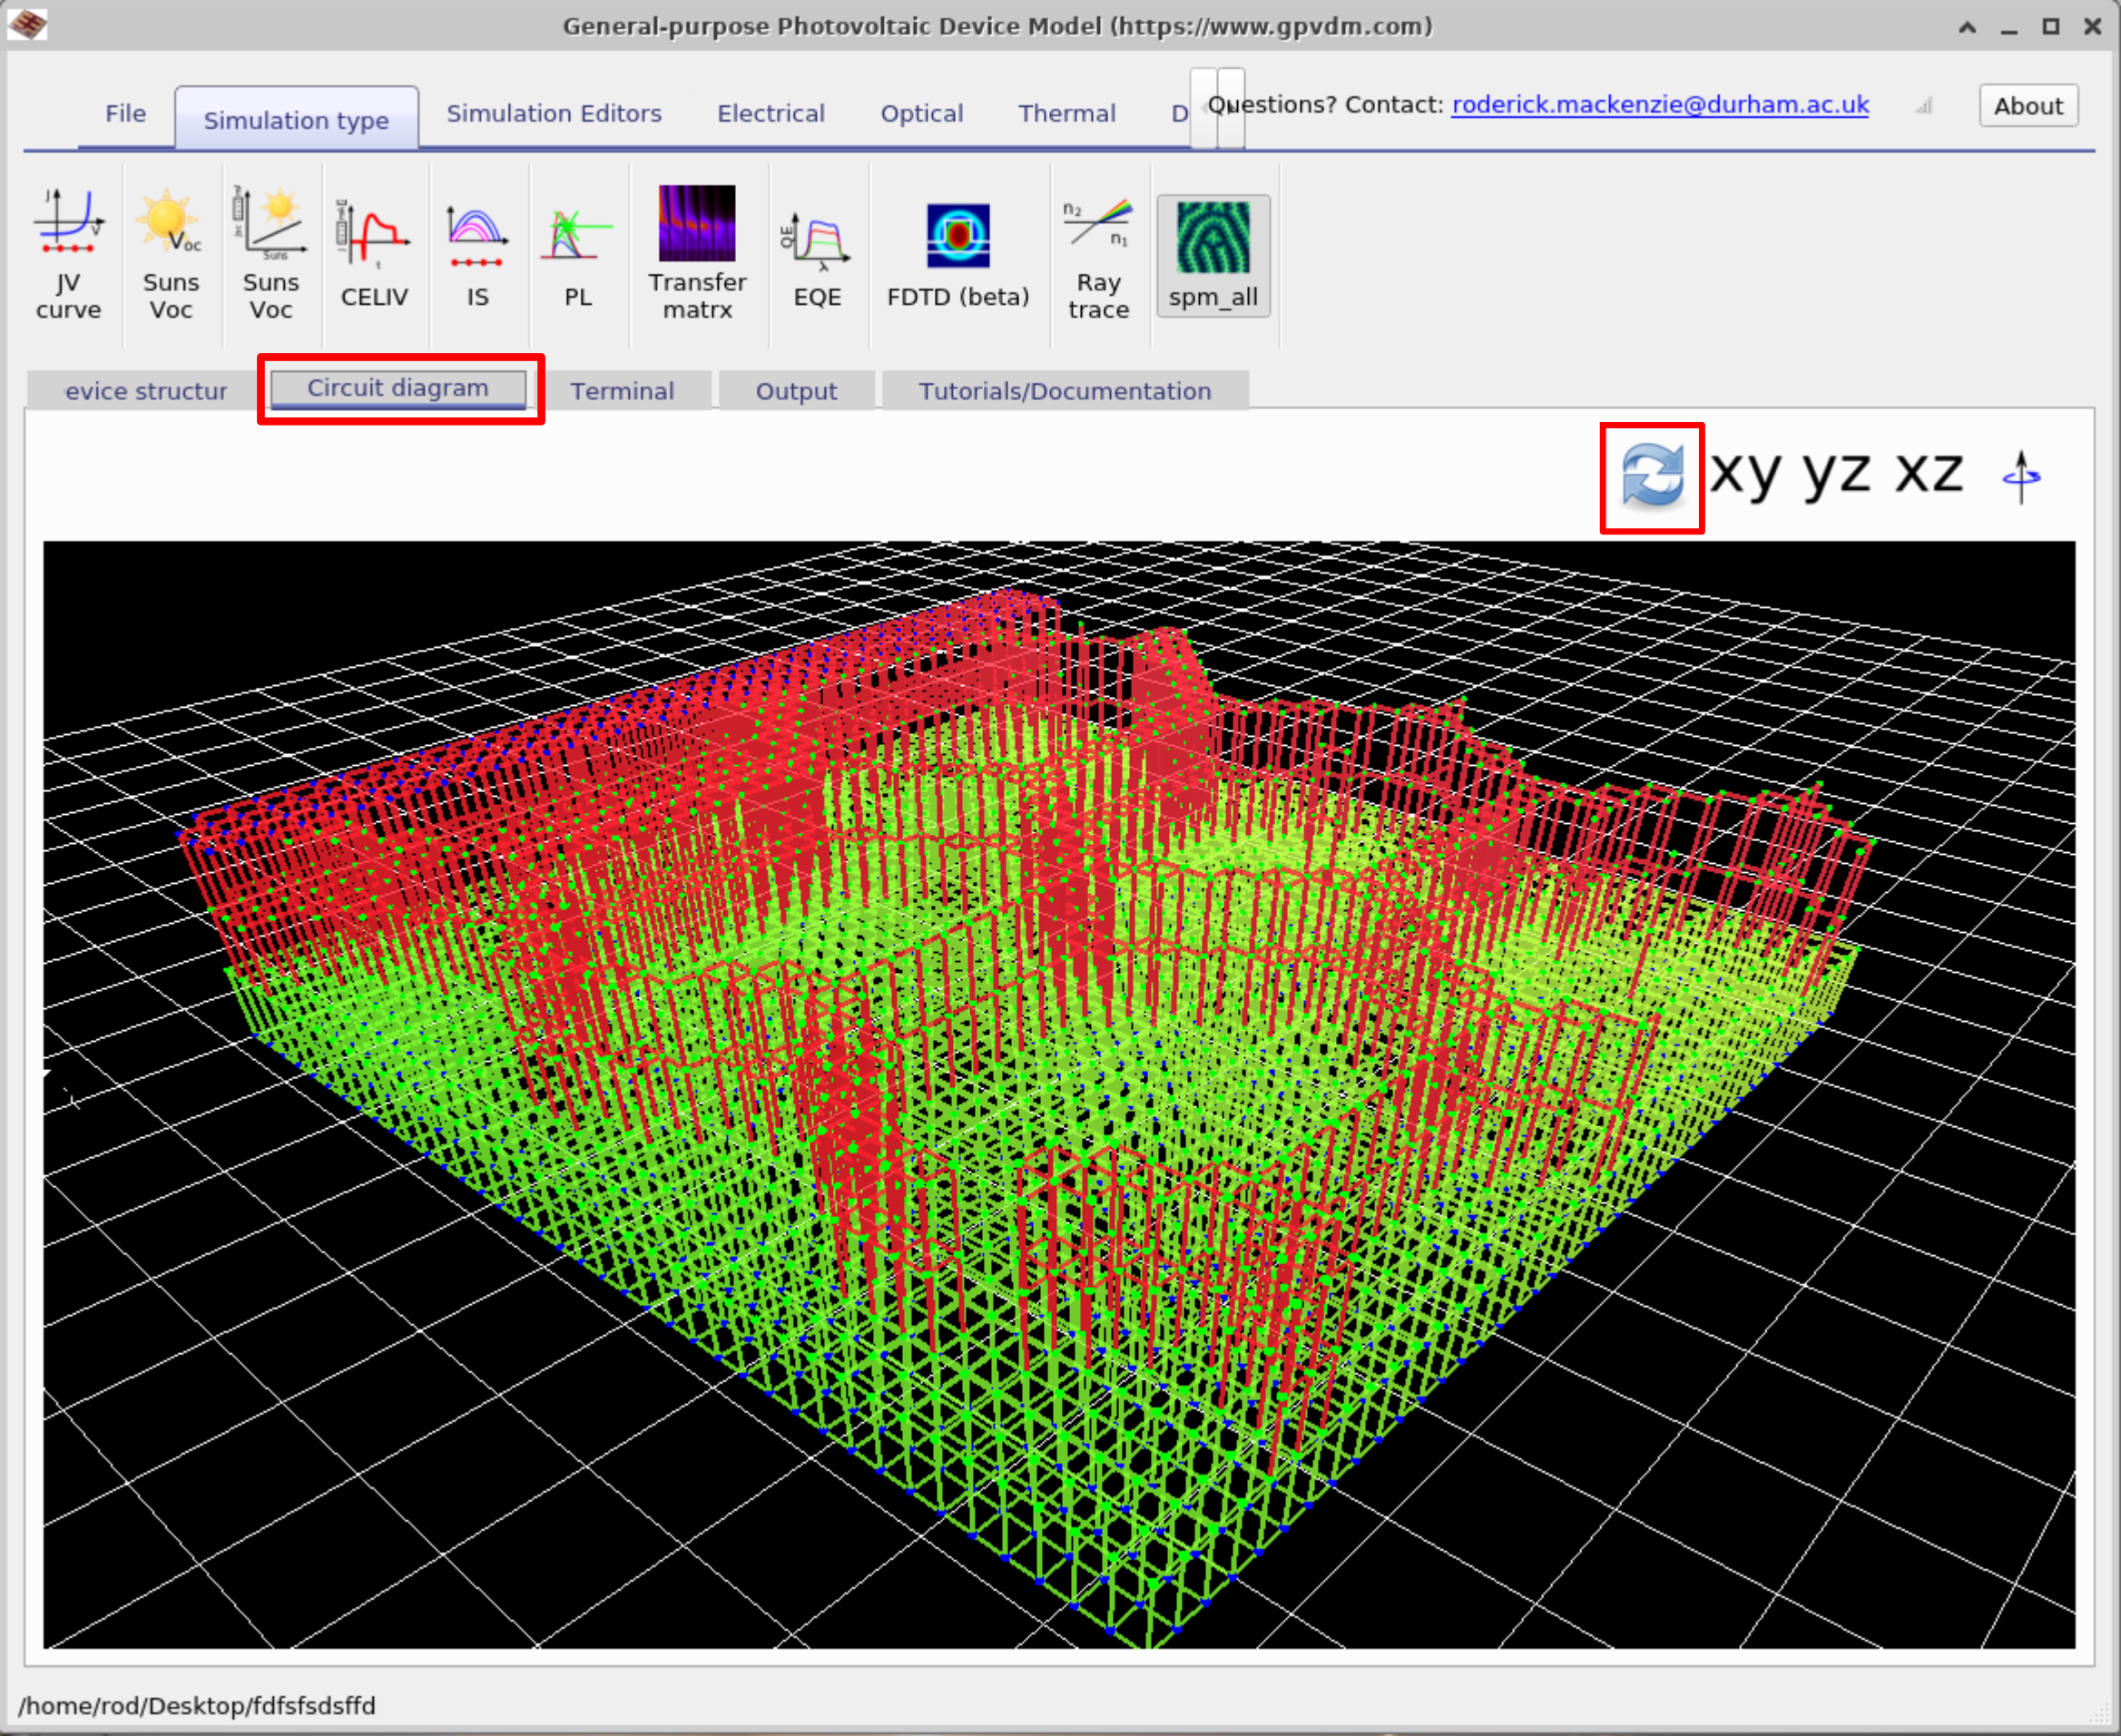
\includegraphics[width=\textwidth]{./images/la_2.png}
\caption{Building the 3D circuit mesh of the contact structure.}
\label{fig:threedcircuitmesh}
\end{figure}

Once this is built we can run a full simulation and calculate the resistance between the bottom of the PEDOT:PSS layer (bottom of the green layer in figure \ref{fig:basecontactsimulation}) and the extracting silver contact (far left yellow strip on the top of figure \ref{fig:basecontactsimulation}). Run the simulation by clicking on the play button in the file ribbon.

\begin{figure}[H]
\centering
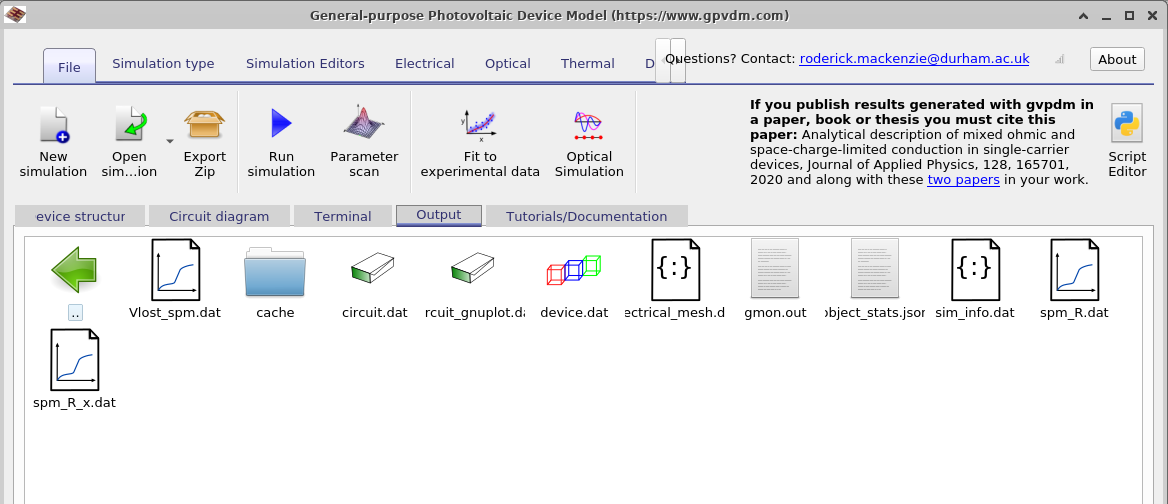
\includegraphics[width=\textwidth]{./images/la_3.png}
\caption{A 1D diagram of the mesh}
\label{fig:circuitoutput}
\end{figure}

The simulation may take a while to run, once it has finished you can open the output files in the \emph{Output} tab, see figure \ref{circuitoutput}.  If you open the file called $spm\_R.dat$ it will show you a resistance map of the structure which can be seen in figure \ref{fig:resistancemap}. Other output files are listed below in table \ref{tab:circuitoutputfiles}.

\begin{figure}[H]
\centering
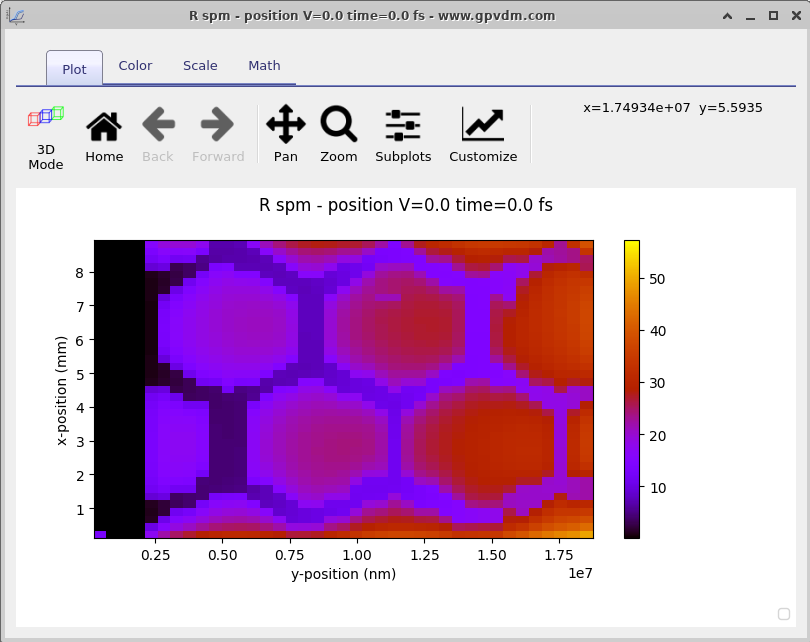
\includegraphics[width=\textwidth]{./images/la_4.png}
\caption{A 2D resistance plot across the surface of the device.}
\label{fig:resistancemap}
\end{figure}

\begin{table}[H]
\begin{center}
\begin{tabular}{ |c|c|c| } 
 \hline
	File name 			& 	Description  \\ 
 \hline
	$spm\_R.dat$ 		&	2D plot of resistance  \\
	$spm\_R\_x.dat$ 		&	A resistance plot down the centre of the device.  \\ 
 \hline
\end{tabular}
\caption{Files produced by the SPM simulaton.}
\label{tab:circuitoutputfiles}
\end{center}
\end{table}

\begin{figure}[H]
\centering
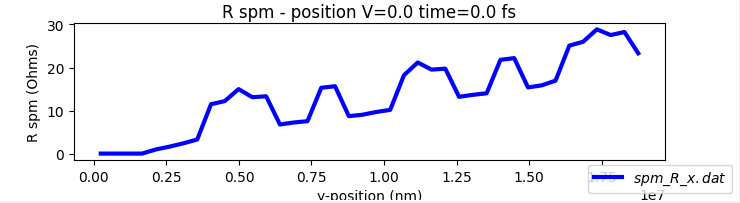
\includegraphics[width=\textwidth]{./images/la_5.png}
\caption{A 1D resistance plot taken through the centre of the device.}
\label{fig:circuittwodplot}
\end{figure}

The scanning probe microscopy editor can be found in the \emph{Simulation Editors} ribbon in the main window. This can be used to select if one scans the entire device or only section of it. The editor can be seen in figure \ref{fig:spmeditor} 
\begin{figure}[H]
\centering
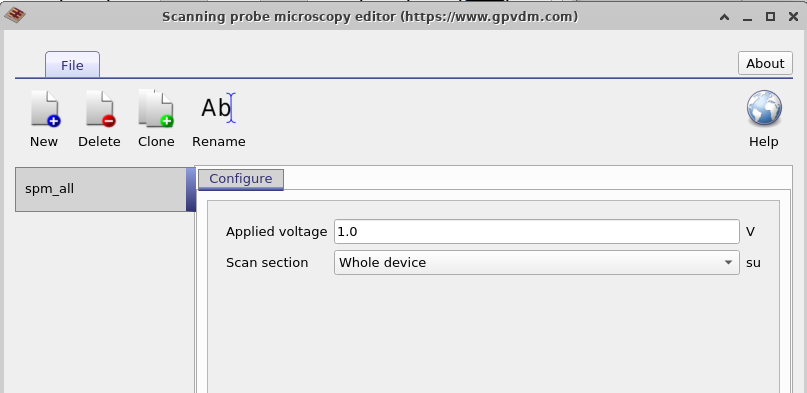
\includegraphics[width=\textwidth]{./images/la_7.png}
\caption{The output files from the simulation.}
\label{fig:spmeditor}
\end{figure}

\section{Simulating large area solar cells}


